\documentclass[aspectratio=1610,onlymath]{beamer}
% \documentclass[aspectratio=1610,onlymath,handout]{beamer}

% Macros used by all lectures, but not necessarily by excercises

% Common notation

\usepackage{amsmath,amssymb,amsfonts}
\usepackage{xspace}

\newcommand{\lectureurl}{https://iccl.inf.tu-dresden.de/web/TheoLog2024}

\DeclareMathAlphabet{\mathsc}{OT1}{cmr}{m}{sc} % Let's have \mathsc since the slide style has no working \textsc

% Dual of "phantom": make a text that is visible but intangible
\newcommand{\ghost}[1]{\raisebox{0pt}[0pt][0pt]{\makebox[0pt][l]{#1}}}

\newcommand{\tuple}[1]{\langle{#1}\rangle}
\newcommand{\defeq}{\mathrel{:=}}

%%% Annotation %%%

\usepackage{color}
\newcommand{\todo}[1]{{\tiny\color{red}\textbf{TODO: #1}}}


\newcommand{\quantor}{\mathord{\reflectbox{$\text{\sf{Q}}$}}} % the generic quantor
\newcommand{\unieq}{\stackrel{.}{=}} % equality sign for unification problems


%%% Old macros below; move when needed

\newcommand{\blank}{\text{\textvisiblespace}} % empty tape cell for TM

% table syntax
\newcommand{\dom}{\textbf{dom}}
\newcommand{\adom}{\textbf{adom}}
\newcommand{\dbconst}[1]{\texttt{"#1"}}
\newcommand{\pred}[1]{\textsf{#1}}
\newcommand{\foquery}[2]{#2[#1]}
\newcommand{\ground}[1]{\textsf{ground}(#1)}
% \newcommand{\foquery}[2]{\{#1\mid #2\}} %% Notation as used in Alice Book
% \newcommand{\foquery}[2]{\tuple{#1\mid #2}}

% logic syntax
\newcommand{\Inter}{\mathcal{I}} %used to denote an interpretation
\newcommand{\Jnter}{\mathcal{J}} %used to denote another interpretation
\newcommand{\Knter}{\mathcal{K}} %used to denote yet another interpretation
\newcommand{\Zuweisung}{\mathcal{Z}} %used to denote a variable assignment

% query languages
\newcommand{\qlang}[1]{{\sf #1}} % Font for query languages
\newcommand{\qmaps}[1]{\textbf{QM}({\sf #1})} % Set of query mappings for a query language

%%% Complexities %%%

\hyphenation{Exp-Time} % prevent "Ex-PTime" (see, e.g. Tobies'01, Glimm'07 ;-)
\hyphenation{NExp-Time} % better that than something else

% \newcommand{\complclass}[1]{{\sc #1}\xspace} % font for complexity classes
\newcommand{\complclass}[1]{\ensuremath{\mathsc{#1}}\xspace} % font for complexity classes

\newcommand{\ACzero}{\complclass{AC$_0$}}
\newcommand{\LogSpace}{\complclass{L}}
\newcommand{\NLogSpace}{\complclass{NL}}
\newcommand{\PTime}{\complclass{P}}
\newcommand{\NP}{\complclass{NP}}
\newcommand{\coNP}{\complclass{coNP}}
\newcommand{\PH}{\complclass{PH}}
\newcommand{\PSpace}{\complclass{PSpace}}
\newcommand{\NPSpace}{\complclass{NPSpace}}
\newcommand{\ExpTime}{\complclass{ExpTime}}
\newcommand{\NExpTime}{\complclass{NExpTime}}
\newcommand{\ExpSpace}{\complclass{ExpSpace}}
\newcommand{\TwoExpTime}{\complclass{2ExpTime}}
\newcommand{\NTwoExpTime}{\complclass{N2ExpTime}}
\newcommand{\ThreeExpTime}{\complclass{3ExpTime}}
\newcommand{\kExpTime}[1]{\complclass{#1ExpTime}}
\newcommand{\kExpSpace}[1]{\complclass{#1ExpSpace}}


%%% Style commands

\newcommand{\quoted}[1]{\texttt{"}{#1}\texttt{"}}
\newcommand{\squote}{\texttt{"}} % straight quote
\newcommand{\Sterm}[1]{\ensuremath{\mathtt{\textcolor{purple}{#1}}}}    % letters in alphabets
\newcommand{\Snterm}[1]{\textsf{\textcolor{darkblue}{#1}}} % nonterminal symbols
\newcommand{\Sntermsub}[2]{\ensuremath{\Snterm{#1}_{\Snterm{#2}}}} % nonterminal symbols
\newcommand{\Slang}[1]{\textbf{\textcolor{black}{#1}}}    % languages
\newcommand{\Slangsub}[2]{\ensuremath{\Slang{#1}_{\Slang{#2}}}}    % languages
% Code
\newcommand{\Scode}[1]{\textbf{#1}}    % reserved words in program listings, e.g., "if"
\newcommand{\Scodelit}[1]{\textcolor{purple}{#1}}    % literals in program listings, e.g., strings
\newcommand{\Scomment}[1]{\textcolor{gray}{#1}}    % comment in program listings
% LOOP and WHILE programs
\newcommand{\Svar}[1]{\texttt{#1}} % variable names
\newcommand{\Svsub}[2]{\ensuremath{\Svar{#1}_{\Svar{#2}}}} % variable names
\newcommand{\Sxsub}[1]{\Svsub{x}{#1}} % variable names
\newcommand{\Sseq}{\texttt{;}}
\newcommand{\SStartLoop}[1]{\Scode{LOOP}~#1~\Scode{DO}~}
\newcommand{\SEndLoop}{\Scode{END}}
\newcommand{\SStartIf}[1]{\Scode{IF}~#1~\Scode{THEN}~}
\newcommand{\SElse}{\Scode{ELSE}}
\newcommand{\SEndIf}{\Scode{END}}
\newcommand{\Svassign}{\texttt{ := }} % variable assignments
\newcommand{\Svneq}{\texttt{!=}\ensuremath{\,}} % inequality operator
\newcommand{\Splus}{\texttt{ + }} % addition operator
\newcommand{\Sminus}{\texttt{ - }} % subtraction operator
\newcommand{\SStartWhile}[1]{\Scode{WHILE}~#1\Svneq\texttt{\Scodelit{0}}~\Scode{DO}~}
\newcommand{\SEndWhile}{\Scode{END}}

\newcommand{\bbfunc}{\boldsymbol{\Sigma}}

\newcommand{\epstrastar}{\mathrel{\mathord{\stackrel{\epsilon}{\to}}{}^*}} % transitive reflexive closure of epsilon transitions in an epslion-NFA

\newcommand{\narrowcentering}[1]{\mbox{}\hfill#1\hfill\mbox{}}

\newcommand{\Smach}[1]{\ensuremath{\mathcal{#1}}}    % machines

\newcommand{\mytrue}{\Scodelit{1}}
\newcommand{\myfalse}{\Scodelit{0}}
% \newcommand{\emptyClause}{\bot}

\newcommand{\Scomplclass}[1]{{\textsc{#1}}\xspace} % font for complexity classes, used on slides where the "too many alphabets" LaTeX error appears when using the correct sc font :-(
% \newcommand{\complclass}[1]{\ensuremath{\mathsc{#1}}} % font for complexity classes


\DeclareMathOperator{\enc}{\mathsf{enc}}

\let\complclass\Scomplclass % prevent "too many math alphabets" error on some slides

%%% General setup and dependencies:

% \usetheme[ddcfooter,nosectionnum]{tud}
\usetheme[nosectionnum,pagenum,noheader]{tud}
% \usetheme[nosectionnum,pagenum]{tud}
\setbeamertemplate{enumerate items}[default]

% Increase body font size to a sane level:
\let\origframetitle\frametitle
% \renewcommand{\frametitle}[1]{\origframetitle{#1}\normalsize}
\renewcommand{\frametitle}[1]{\origframetitle{#1}\fontsize{10pt}{13.2}\selectfont}
\setbeamerfont{itemize/enumerate subbody}{size=\small} % tud defaults to scriptsize!
\setbeamerfont{itemize/enumerate subsubbody}{size=\small}
% \setbeamerfont{normal text}{size=\small}
% \setbeamerfont{itemize body}{size=\small}

\renewcommand{\emph}[1]{\textbf{#1}}

\def\arraystretch{1.3}% Make tables even less cramped vertically

\usepackage[ngerman]{babel}
\usepackage[utf8]{inputenc}
\usepackage[T1]{fontenc}

%\usepackage{graphicx}
\usepackage[export]{adjustbox} % loads graphicx
\usepackage{import}
\usepackage{stmaryrd}
\usepackage[normalem]{ulem} % sout command
% \usepackage{times}
\usepackage{txfonts}
\usepackage{array}

% \usepackage[perpage]{footmisc} % reset footnote counter on each page -- fails with beamer (footnotes gone)
\usepackage{perpage}  % reset footnote counter on each page
\MakePerPage{footnote}

\usepackage{tikz}
\usetikzlibrary{arrows,positioning,decorations.pathreplacing}
% Inspired by http://www.texample.net/tikz/examples/hand-drawn-lines/
\usetikzlibrary{decorations.pathmorphing}
\pgfdeclaredecoration{penciline}{initial}{
    \state{initial}[width=+\pgfdecoratedinputsegmentremainingdistance,
    auto corner on length=1mm,]{
        \pgfpathcurveto%
        {% From
            \pgfqpoint{\pgfdecoratedinputsegmentremainingdistance}
                      {\pgfdecorationsegmentamplitude}
        }
        {%  Control 1
        \pgfmathrand
        \pgfpointadd{\pgfqpoint{\pgfdecoratedinputsegmentremainingdistance}{0pt}}
                    {\pgfqpoint{-\pgfdecorationsegmentaspect
                     \pgfdecoratedinputsegmentremainingdistance}%
                               {\pgfmathresult\pgfdecorationsegmentamplitude}
                    }
        }
        {%TO
        \pgfpointadd{\pgfpointdecoratedinputsegmentlast}{\pgfpoint{1pt}{1pt}}
        }
    }
    \state{final}{}
}
\tikzset{handdrawn/.style={decorate,decoration=penciline}}
\tikzset{every shadow/.style={fill=none,shadow xshift=0pt,shadow yshift=0pt}}
% \tikzset{module/.append style={top color=\col,bottom color=\col}}

% Use to make Tikz attributes with Beamer overlays
% http://tex.stackexchange.com/a/6155
\tikzset{onslide/.code args={<#1>#2}{%
  \only<#1| handout:0>{\pgfkeysalso{#2}}
}}
\tikzset{onslideprint/.code args={<#1>#2}{%
  \only<#1>{\pgfkeysalso{#2}}
}}

%%% Title -- always set this first

\newcommand{\defineTitle}[3]{
	\newcommand{\lectureindex}{#1}
	\title{Theoretische Informatik und Logik}
	\subtitle{\href{\lectureurl}{#1. Vorlesung: #2}}
	\author{\href{https://iccl.inf.tu-dresden.de/web/Markus_Kr\%C3\%B6tzsch}{Markus Kr\"{o}tzsch}\\[1ex]Professur Wissensbasierte Systeme}
	\date{#3}
	\datecity{TU Dresden}
% 	\institute{CC-By 3.0, sofern keine anderslautenden Bildrechte angegeben sind}
}

%%% Table of contents:

\RequirePackage{ifthen}

\newcommand{\highlight}[2]{%
	\ifthenelse{\equal{#1}{\lectureindex}}{\alert{#2}}{#2}%
}

\def\myspace{-0.7ex}
\newcommand{\printtoc}{
\begin{tabular}{r@{$\quad$}l}
\highlight{1}{1.} & \highlight{1}{Willkommen/Einleitung formale Sprachen}\\[\myspace]
\highlight{2}{2.} & \highlight{2}{Grammatiken und die Chomsky-Hierarchie}\\[\myspace]
\highlight{3}{3.} & \highlight{3}{Endliche Automaten}\\[\myspace]
\highlight{4}{4.} & \highlight{4}{Complexity of FO query answering}\\[\myspace]
\highlight{5}{5.} & \highlight{5}{Conjunctive queries}\\[\myspace]
\highlight{6}{6.} & \highlight{6}{Tree-like conjunctive queries}\\[\myspace]
\highlight{7}{7.} & \highlight{7}{Query optimisation}\\[\myspace]
\highlight{8}{8.} & \highlight{8}{Conjunctive Query Optimisation / First-Order~Expressiveness}\\[\myspace]
\highlight{9}{9.} & \highlight{9}{First-Order~Expressiveness / Introduction to Datalog}\\[\myspace]
\highlight{10}{10.} & \highlight{10}{Expressive Power and Complexity of Datalog}\\[\myspace]
\highlight{11}{11.} & \highlight{11}{Optimisation and Evaluation of Datalog}\\[\myspace]
\highlight{12}{12.} & \highlight{12}{Evaluation of Datalog (2)}\\[\myspace]
\highlight{13}{13.} & \highlight{13}{Graph Databases and Path Queries}\\[\myspace]
\highlight{14}{14.} & \highlight{14}{Outlook: database theory in practice}
\end{tabular}
}

\newcommand{\overviewslide}{%
\begin{frame}\frametitle{Overview}
\printtoc
\medskip

Siehe \href{\lectureurl}{course homepage [$\Rightarrow$ link]} for more information and materials
\end{frame}
}

%%% Colours:
\usepackage{xcolor,colortbl}
\definecolor{redhighlights}{HTML}{FFAA66}
\definecolor{lightblue}{HTML}{55AAFF}
\definecolor{lightred}{HTML}{FF5522}
\definecolor{lightpurple}{HTML}{DD77BB}
\definecolor{lightgreen}{HTML}{55FF55}
\definecolor{lightgray}{HTML}{CCCCCC}
\definecolor{darkred}{HTML}{CC4411}
\definecolor{darkblue}{HTML}{176FC0}%{1133AA}
\definecolor{nightblue}{HTML}{2010A0}%{1133AA}
\definecolor{alert}{HTML}{176FC0}
\definecolor{darkgreen}{HTML}{36AB14}
\definecolor{strongyellow}{HTML}{FFE219}
\definecolor{devilscss}{HTML}{666666}

\newcommand{\redalert}[1]{\textcolor{darkred}{#1}}

%%% Slide layout commands:

\newcommand{\sectionSlide}[1]{
\frame{\begin{center}
\LARGE
#1
\end{center}}
}
\newcommand{\sectionSlideNoHandout}[1]{
\frame<handout:0>{\begin{center}
\LARGE
#1
\end{center}}
}

\newcommand{\mydualbox}[3]{%
 \begin{minipage}[t]{#1}
 \begin{beamerboxesrounded}[upper=block title,lower=block body,shadow=true]%
    {\centering\usebeamerfont*{block title}#2}%
    \raggedright%
    \usebeamerfont{block body}
%     \small
    #3%
  \end{beamerboxesrounded}
  \end{minipage}
}
%
\newcommand{\myheaderbox}[2]{%
 \begin{minipage}[t]{#1}
 \begin{beamerboxesrounded}[upper=block title,lower=block title,shadow=true]%
    {\centering\usebeamerfont*{block title}\rule{0pt}{2.6ex} #2}%
  \end{beamerboxesrounded}
  \end{minipage}
}

\newcommand{\mycontentbox}[2]{%
 \begin{minipage}[t]{#1}%
 \begin{beamerboxesrounded}[upper=block body,lower=block body,shadow=true]%
    {\centering\usebeamerfont*{block body}\rule{0pt}{2.6ex}#2}%
  \end{beamerboxesrounded}
  \end{minipage}
}

\newcommand{\mylcontentbox}[2]{%
 \begin{minipage}[t]{#1}%
 \begin{beamerboxesrounded}[upper=block body,lower=block body,shadow=true]%
    {\flushleft\usebeamerfont*{block body}\rule{0pt}{2.6ex}#2}%
  \end{beamerboxesrounded}
  \end{minipage}
}

% label=180:{\rotatebox{90}{{\footnotesize\textcolor{darkgreen}{Beispiel}}}}
% \hspace{-8mm}\ghost{\raisebox{-7mm}{\rotatebox{90}{{\footnotesize\textcolor{darkgreen}{Beispiel}}}}}\hspace{8mm}
\newcommand{\examplebox}[1]{%
	\begin{tikzpicture}[decoration=penciline, decorate]
		\pgfmathsetseed{1235}
		\node (n1) [decorate,draw=darkgreen, fill=darkgreen!10,thick,align=left,text width=\linewidth, inner ysep=2mm, inner xsep=2mm] at (0,0) {#1};
% 		\node (n2) [align=left,text width=\linewidth,inner sep=0mm] at (n1.92) {{\footnotesize\raisebox{3mm}{\textcolor{darkgreen}{Beispiel}}}};
% 		\node (n2) [decorate,draw=darkgreen, fill=darkgreen!10,thick, align=left,text width=\linewidth,inner sep=2mm] at (n1.90) {{\footnotesize\raisebox{0mm}{\textcolor{darkgreen}{Beispiel}}}};
	\end{tikzpicture}%
}%

\newcommand{\codebox}[1]{%
	\begin{tikzpicture}[decoration=penciline, decorate]
		\pgfmathsetseed{1236}
		\node (n1) [decorate,draw=strongyellow, fill=strongyellow!10,thick,align=left,text width=\linewidth, inner ysep=2mm, inner xsep=2mm] at (0,0) {#1};
	\end{tikzpicture}%
}%

\newcommand{\defbox}[1]{%
	\begin{tikzpicture}[decoration=penciline, decorate]
		\pgfmathsetseed{1237}
		\node (n1) [decorate,draw=darkred, fill=darkred!10,thick,align=left,text width=\linewidth, inner ysep=2mm, inner xsep=2mm] at (0,0) {#1};
	\end{tikzpicture}%
}%

\newcommand{\theobox}[1]{%
	\begin{tikzpicture}[decoration=penciline, decorate]
		\pgfmathsetseed{1240}
		\node (n1) [decorate,draw=darkblue, fill=darkblue!10,thick,align=left,text width=\linewidth, inner ysep=2mm, inner xsep=2mm] at (0,0) {#1};
	\end{tikzpicture}%
}%

\newcommand{\anybox}[2]{%
	\begin{tikzpicture}[decoration=penciline, decorate]
		\pgfmathsetseed{1240}
		\node (n1) [decorate,draw=#1, fill=#1!10,thick,align=left,text width=\linewidth, inner ysep=2mm, inner xsep=2mm] at (0,0) {#2};
	\end{tikzpicture}%
}%


\newsavebox{\mybox}%
\newcommand{\doodlebox}[2]{%
\sbox{\mybox}{#2}%
	\begin{tikzpicture}[decoration=penciline, decorate]
		\pgfmathsetseed{1238}
		\node (n1) [decorate,draw=#1, fill=#1!10,thick,align=left,inner sep=1mm] at (0,0) {\usebox{\mybox}};
	\end{tikzpicture}%
}%


\defineTitle{4}{Das Halteproblem und Reduktionen}{18. April 2024}

\begin{document}

\maketitle

% \begin{frame}\frametitle{Ankündigung}
% 
% Die Übungsgruppen am 1. Mai werden verschoben:
% 
% \begin{itemize}
% \item Mittwoch 2.5. in der 5.DS in APB/3027
% \item Donnerstag 3.5. in der 6.DS in APB/3027
% \end{itemize}
% 
% Studierende aus den den betroffenen Übungsgruppen sollten nach
% Möglichkeit die o.g. Ausweichtermine nutzen, können aber auch in eine
% der anderen Übungsgruppen die in der Woche stattfinden ausweichen.
% 
% \end{frame}


\sectionSlide{LOOP und WHILE, Reprise}

\begin{frame}\frametitle{Zusammenfassung LOOP und WHILE}

\emph{LOOP-Programme}
\begin{itemize}
\item Terminieren immer
\item Können fast alle praktisch relevanten Funktionen berechnen
\item Können nicht jede berechenbare Funktion berechnen, z.B. Ackermann-Funktion, Sudan-Funktion, LOOP-Busy-Beaver
\end{itemize}
\bigskip

\emph{WHILE-Programme}
\begin{itemize}
\item Verallgemeinern LOOP
\item Terminieren nicht immer
\item Können alle berechenbaren totalen und partiellen Funktionen berechnen
\end{itemize}

\end{frame}

\begin{frame}\frametitle{Die Kraft des LOOP}

Auf der vorigen Folie steht: "`LOOP-Programme können fast alle praktisch relevanten Funktionen berechnen."'
\medskip

\redalert{Stimmt das wirklich?}
\bigskip\pause

\emph{Idee:} Die Schleife $\SStartWhile{\Svar{x}}P~\SEndWhile$ kann mit dem folgenden LOOP-Programm simuliert werden:\medskip

\codebox{{\tt
\SStartLoop{\Svar{max}}\\
~~~\SStartIf{\Svar{x}\Svneq\Scodelit{0}}\\
~~~~~~P\\
~~~\SEndIf\\
\SEndLoop
}}\pause

wenn man den Wert von $\Svar{max}$ so setzt, dass er \alert{mindestens} so groß ist
wie die maximale Anzahl von Wiederholungen der simulierten WHILE-Schleife.

\end{frame}

\begin{frame}\frametitle{LOOP kann WHILE simulieren}

\alert{Erkenntnis:} LOOP kann WHILE für beliebig viele Schritte simulieren -- man muss nur wissen, wie viele Schritte benötigt werden.
\bigskip

\redalert{Kann man das ausrechnen?}\pause{} \alert{Ja!}\bigskip

\theobox{\emph{Satz:} Für ein beliebiges WHILE-Programm $P$ sei $\textsf{max}_P(n_1,\ldots,n_k)$
die maximale Anzahl an Schleifendurchläufen, die $P$ bei der Eingabe $n_1,\ldots,n_k$
abarbeitet, oder undefiniert, wenn $P$ bei dieser Eingabe nicht terminiert.
Diese partielle Funktion $\textsf{max}_P:\mathbb{N}^k\to\mathbb{N}$ ist berechenbar.
}
\emph{Beweisskizze:} Man kann $P$ leicht so modifizieren, dass es die Maximalzahl der Schleifendurchläufe bestimmt und ausgibt.\qed\medskip\pause

\alert{Wo ist der Haken?}\pause\medskip

Die Funktion $\textsf{max}_P$ ist zwar berechenbar, aber im Allgemeinen nicht LOOP-berechenbar.

\end{frame}

\begin{frame}\frametitle{Was kann LOOP?}

Es gibt aber viele Fälle, in denen man (eine obere Schranke von) $\textsf{max}_P$ LOOP-berechnen kann:

\theobox{\emph{Satz:} Die folgenden Funktionen sind LOOP-berechenbar:
\begin{itemize}
\item $n\cdot \Svar{x}$ für beliebige natürliche Zahlen $n$
\item $\Svar{x}^n$ für beliebige natürliche Zahlen $n$
\item $n^{\Svar{x}}$ für beliebige natürliche Zahlen $n$
\item $n^{.^{.^{.^{n^{\Svar{x}}}}}}$ für beliebig hohe Türme von Exponenten $n$
\end{itemize}
}\bigskip\pause

\theobox{\emph{Korollar:} Jeder Algorithmus, der in Zeit $O(n^{.^{.^{.^{n^{\Svar{x}}}}}})$ -- oder weniger -- läuft, berechnet eine LOOP-berechenbare Funktion. Insbesondere sind alle polynomiellen, exponentiellen oder mehrfach exponentiellen Algorithmen in LOOP implementierbar.\\[-0.6ex]~
}

\end{frame}

\sectionSlide{Universalität}

\begin{frame}\frametitle{Die Universalmaschine}

Eine erste wichtige Beobachtung Turings war, dass TMs stark genug sind um andere TMs zu simulieren:
\bigskip

\begin{enumerate}[{Schritt} 1:]
\item Kodiere Turingmaschinen $\Smach{M}$ als Wörter $\textsf{enc}(\Smach{M})$
\item Konstruiere eine \redalert{universelle Turingmaschine} $\Smach{U}$, die $\textsf{enc}(\Smach{M})$ als Eingabe erhält und dann die Berechnung von $\Smach{M}$ simuliert
\end{enumerate}

\end{frame}

\begin{frame}\frametitle{Schritt 1: Turingmaschinen kodieren}

Jede vernünftige Kodierung einer TM $\Smach{M}=\tuple{Q,\Sigma,\Gamma,\delta,q_0,F}$ ist nutzbar, zum Beispiel die folgende (für DTMs):\medskip

\anybox{gray}{%
\footnotesize\vspace{-2ex}%
\begin{itemize}
\item Wir verwenden das Alphabet $\{\Sterm{0},\Sterm{1},\Sterm{\#}\}$
\item Zustände werden in beliebiger Reihenfolge nummeriert (mit Startzustand $q_0$) und binär kodiert:\\
	$Q=\{q_0,\ldots,q_n\}$ $\leadsto$ $\textsf{enc}(Q)=\textsf{bin}(0)\Sterm{\#}\cdots\Sterm{\#}\textsf{bin}(n)$
\item Wir kodieren auch $\Gamma$ und die Bewegungsrichtungen $\{R,L,N\}$ binär
\item Ein Übergang $\delta(q_i,\sigma_n)=\tuple{q_j,\sigma_m,D}$ wird als 5-Tupel kodiert:\\
	 $\textsf{enc}(q_i,\sigma_n)=\textsf{bin}(i)\Sterm{\#}\textsf{bin}(n)\Sterm{\#}\textsf{bin}(j)\Sterm{\#}\textsf{bin}(m)\Sterm{\#}\textsf{bin}(D)$
\item Die Übergangsfunktion wird kodiert als Liste aller dieser Tupel, getrennt mit $\Sterm{\#}$:
	$\textsf{enc}(\delta)=\big(\textsf{enc}(q_i,\sigma_n)\Sterm{\#}\big)_{q_i\in Q, \sigma_i\in\Gamma}$
\item Insgesamt setzten wir $\textsf{enc}(\Smach{M})=\textsf{enc}(Q)\Sterm{\#}\Sterm{\#}\textsf{enc}(\Sigma)\Sterm{\#}\Sterm{\#}\textsf{enc}(\Gamma)\Sterm{\#}\Sterm{\#}\textsf{enc}(\delta)\Sterm{\#}\Sterm{\#}\textsf{enc}(F)$
\end{itemize}}

Passend dazu kann man auch beliebige Wörter kodieren:

\anybox{gray}{%
\footnotesize\vspace{-2ex}%
\begin{itemize}
\item Für ein Wort $w=a_1\cdots a_{\ell}$ setzen wir $\textsf{enc}(w)=\textsf{bin}(a_1)\Sterm{\#}\cdots\Sterm{\#}\textsf{bin}(a_{\ell})$
\end{itemize}
}

\end{frame}

\begin{frame}\frametitle{Schritt 2: Die universelle Turingmaschine}

Wir definieren die universelle TM $\Smach{U}$ als Mehrbandturingmaschine:
\begin{enumerate}[{Band} 1:]
\item Eingabeband von $\Smach{U}$: enthält $\textsf{enc}(\Smach{M})\Sterm{\#\#}\textsf{enc}(w)$
\item Arbeitsband von $\Smach{U}$
\item Speichert den Zustand der simulierten Turingmaschine
\item Arbeitsband der simulierten Turingmaschine
\end{enumerate}
\bigskip\pause

Die Arbeitsweise von $\Smach{U}$ ist leicht skizziert:
\anybox{gray}{%
\footnotesize\vspace{-2ex}%
\begin{itemize}
\item $\Smach{U}$ prüft Eingabe, kopiert $\textsf{enc}(w)$ auf Band 4, verschiebt den Kopf auf Band 4 zum Anfang und initialisiert Band 3 mit $\textsf{enc}(0)$.
\item In jedem Schritt liest $\Smach{U}$ ein (kodiertes) Zeichen von der aktuellen Kopfposition auf Band (4), sucht für den simulierten Zustand (Band~3) einen passenden Übergang in $\textsf{enc}(\Smach{M})$ auf Band 1:
	\begin{itemize}\footnotesize
	\item Übergang gefunden: setze Band 3 auf den neuen Zustand; ersetzt das kodierte Zeichen auf Band 4 durch das neue Zeichen; verschiebe den Kopf auf Band 4 entsprechend
	\item Übergang nicht gefunden: nimm Endzustand ein, falls der Zustand von Band 3 Endzustand in $\textsf{enc}(\Smach{M})$ ist; halte
	\end{itemize}
\end{itemize}
}

\end{frame}

\begin{frame}\frametitle{Die Theorie der Software}

\theobox{\emph{Satz:} Es gibt eine \redalert{universelle Turingmaschine} $\Smach{U}$, die für Eingaben der Form $\textsf{enc}(\Smach{M})\Sterm{\#}\Sterm{\#}\textsf{enc}(w)$ das Verhalten der DTM $\Smach{M}$ auf $w$ simuliert:
\begin{itemize}
\item Falls $\Smach{M}$ auf $w$ hält, dann hält $\Smach{U}$ auf $\textsf{enc}(\Smach{M})\Sterm{\#}\Sterm{\#}\textsf{enc}(w)$ mit dem gleichen Ergebnis
\item Falls $\Smach{M}$ auf $w$ nicht hält, dann hält $\Smach{U}$ auf $\textsf{enc}(\Smach{M})\Sterm{\#}\Sterm{\#}\textsf{enc}(w)$ ebenfalls nicht
\end{itemize}}\bigskip

Unsere Konstruktion ist für DTMs, die Sprachen erkennen -- DTMs, die Funktionen berechnen, können ähnlich simuliert werden.\bigskip\pause

\alert{Praktische Konsequenzen:}
\begin{itemize}
\item Universalrechner sind möglich
\item Wir müssen nicht für jede neue Anwendung einen neuen Computer anschaffen
\item Es gibt Software
\end{itemize}


\end{frame}

\sectionSlide{Unentscheidbare Probleme und Reduktionen}

\begin{frame}\frametitle{Das Halteproblem}

Ein klassisches unentscheidbares Problem ist das Halteproblem:
\bigskip

\defbox{Das \redalert{Halteproblem} besteht in der folgenden Frage:\\
\hspace{1cm}Gegeben eine TM $\Smach{M}$ und ein Wort $w$,\\\hspace{1cm}wird $\Smach{M}$ für die Eingabe $w$ jemals anhalten?}\bigskip\pause

Wir können das Halteproblem formal als Entscheidungsproblem ausdrücken, wenn wir $\Smach{M}$ und $w$ kodieren:\bigskip

\defbox{Das \redalert{Halteproblem} ist das Wortproblem für die Sprache\\[1ex]
\narrowcentering{
$\Slang{P}_{\textsf{Halt}} = \{\textsf{enc}(\Smach{M})\Sterm{\#}\Sterm{\#}\textsf{enc}(w)\mid \text{$\Smach{M}$ hält bei Eingabe $w$}\}$,
}\\[1ex]
wobei $\textsf{enc}(\Smach{M})$ und $\textsf{enc}(w)$ geeignete Kodierungen von $\Smach{M}$ und $w$ sind, so dass $\Sterm{\#}\Sterm{\#}$ als Trennwort verwendet werden kann.}\medskip

\alert{Anmerkung:} Falsch kodierte Eingaben werden hier auch abgelehnt.

\end{frame}

\begin{frame}[t]\frametitle{"`Beweis"' durch Intuition}

\theobox{\emph{Satz:} Das Halteproblem $\Slang{P}_{\textsf{Halt}}$ ist unentscheidbar.}\pause

\emph{"`Beweis:"'} Das Gegenteil wäre zu schön um wahr zu sein. Viele ungelöste Probleme
könnte man damit direkt lösen.\bigskip\pause

\examplebox{\emph{Beispiel:} Die Goldbachsche Vermutung (Christian Goldbach, 1742) besagt, dass jede gerade Zahl $n\geq 4$ die Summe zweier Primzahlen ist. Zum Beispiel ist $4=2+2$ und $100=47+53$.}\pause

Man kann leicht einen Algorithmus \Smach{A} angeben, der die Goldbachsche Vermuting systematisch verifiziert, d.h., für alle geraden Zahlen ab $4$ testet:
\begin{itemize}
\item Erfolg: teste die nächste gerade Zahl
\item Misserfolg: terminiere mit Meldung "`Goldbach hat sich geirrt!"'
\end{itemize}

Die Frage "`Wird \Smach{A} halten?"' ist gleichbedeutend mit der Frage\\"`Gilt die Goldbachsche Vermutung nicht?"'
\ghost{\hspace{7.4cm}\rotatebox{90}{\textcolor{devilscss}{{\tiny Vgl. 3. Übung, Aufg. 4: Mit $\Slang{P}_{\textsf{Halt}}$ kann man alle semi-entscheidbaren Probleme lösen}}}}

\end{frame}

\begin{frame}\frametitle{Abschweifung}

\begin{center}
\large Ist die Goldbachsche Vermutung entscheidbar?
\end{center}

\end{frame}

\begin{frame}[t]\frametitle{Beweis durch "`Diagonalisierung"'}

\theobox{\emph{Satz:} Das Halteproblem $\Slang{P}_{\textsf{Halt}}$ ist unentscheidbar.}\pause

\emph{Beweis:} Per Widerspruch: Wir nehmen an, dass es einen Entscheider $\Smach{H}$ für das Halteproblem gibt.\pause
\bigskip

Dann kann man eine TM $\Smach{D}$ konstruieren, die folgendes tut:
\begin{enumerate}[(1)]
\item Prüfe, ob die Eingabe eine TM-Kodierung $\textsf{enc}(\Smach{M})$ ist
\item Simuliere $\Smach{H}$ auf der Eingabe $\textsf{enc}(\Smach{M})\Sterm{\#\#}\textsf{enc}(\textsf{enc}(\Smach{M}))$, d.h. prüfe, ob $\Smach{M}$ auf $\textsf{enc}(\Smach{M})$ hält
\item Falls ja, dann gehe in eine Endlosschleife;\\ falls nein, dann halte und akzeptiere
\end{enumerate}
\bigskip\pause

% \alert{Wer rasiert den Barbier?}
\alert{Akzeptiert $\Smach{D}$ die Eingabe $\textsf{enc}(\Smach{D})$?}\pause\\[1ex]

\narrowcentering{$\Smach{D}$ hält und akzeptiert $\quad$ genau dann wenn $\quad$ $\Smach{D}$ nicht hält}\\[1ex]

Widerspruch.\qed

\end{frame}

\begin{frame}\frametitle{Diagonalisierung, graphische Darstellung}

\begin{minipage}{5cm}
\emph{Bekannt:} Eine Maschine hält auf einem Input oder nicht:\bigskip

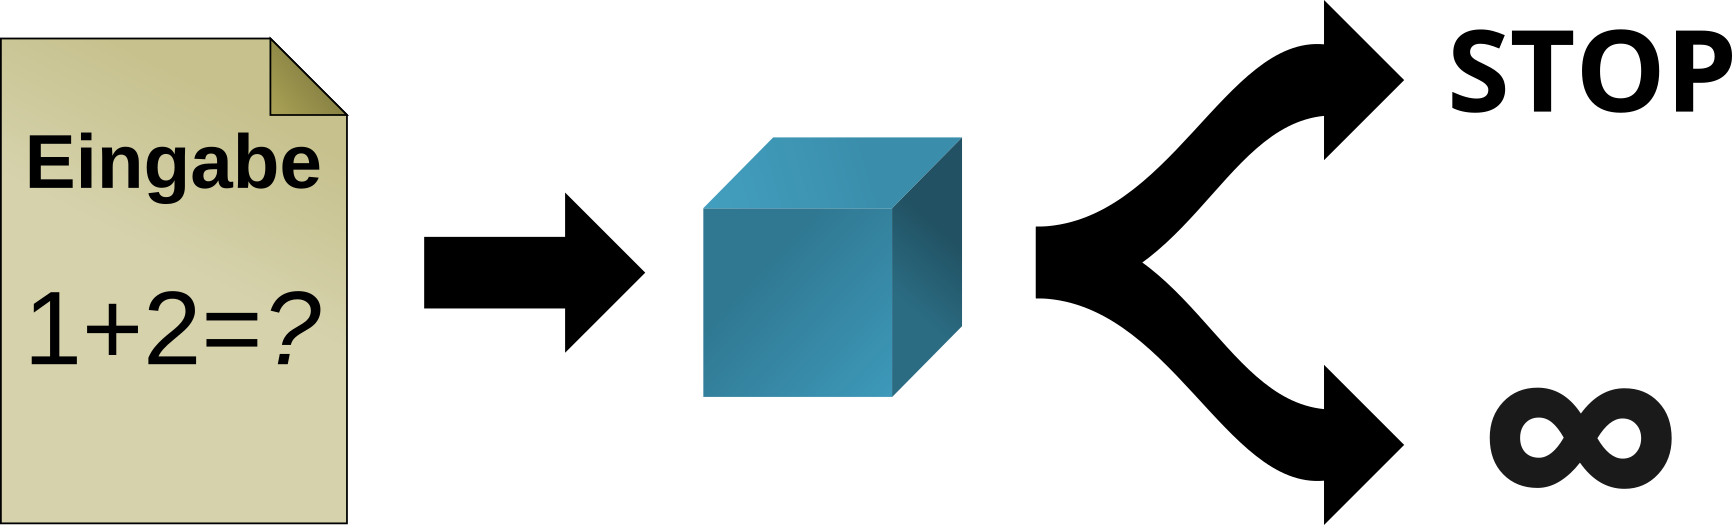
\includegraphics[width=5cm]{images/halting-tm}\bigskip

\emph{Annahme:} Es gibt eine Maschine, die Halten entscheidet:\bigskip

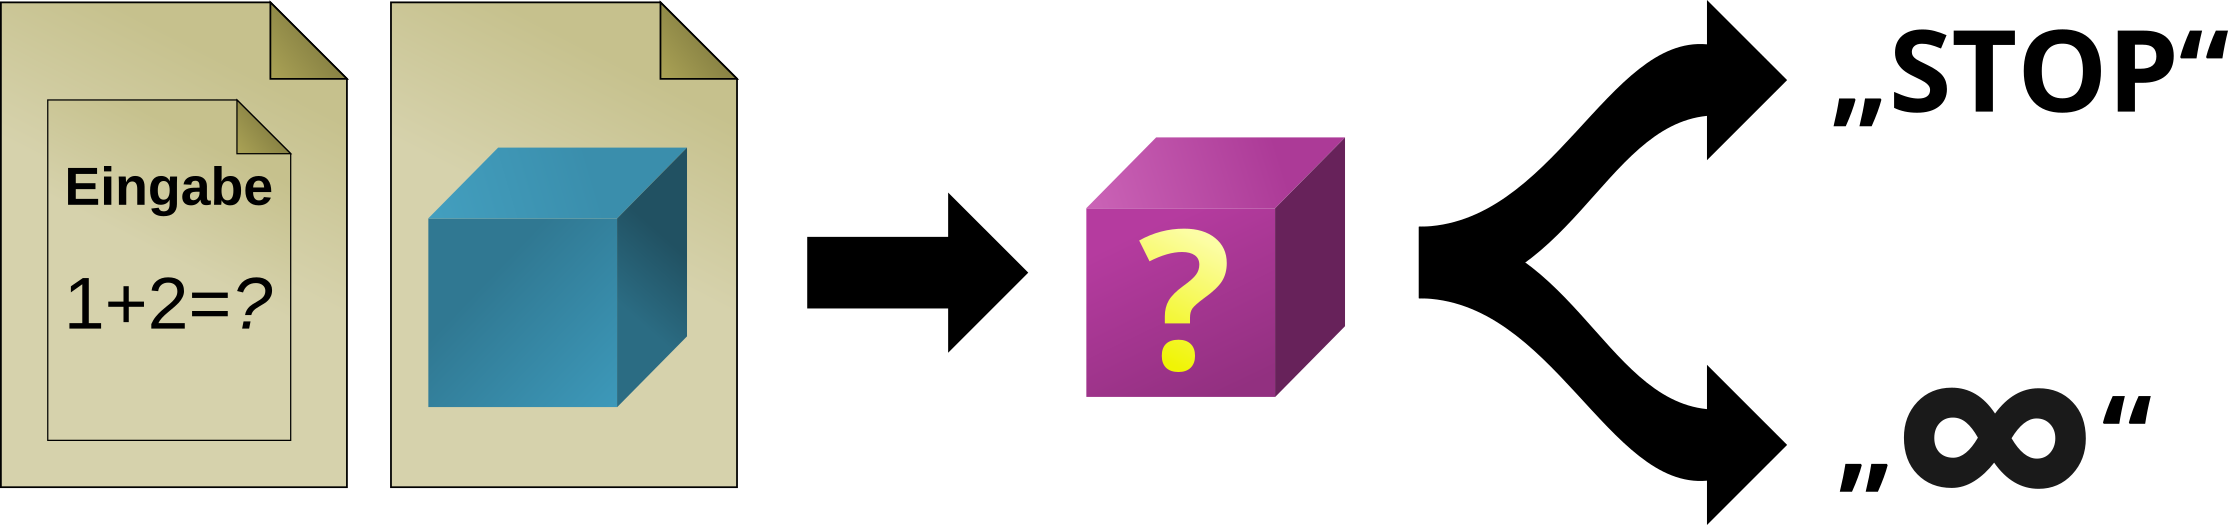
\includegraphics[width=5cm]{images/halting-oracle}

\vspace{0.9cm}~
\end{minipage}\hfill%
\begin{minipage}{7cm}

\emph{Bauplan Diagonalisierungsmaschine:}\bigskip

~\hspace{0.5cm}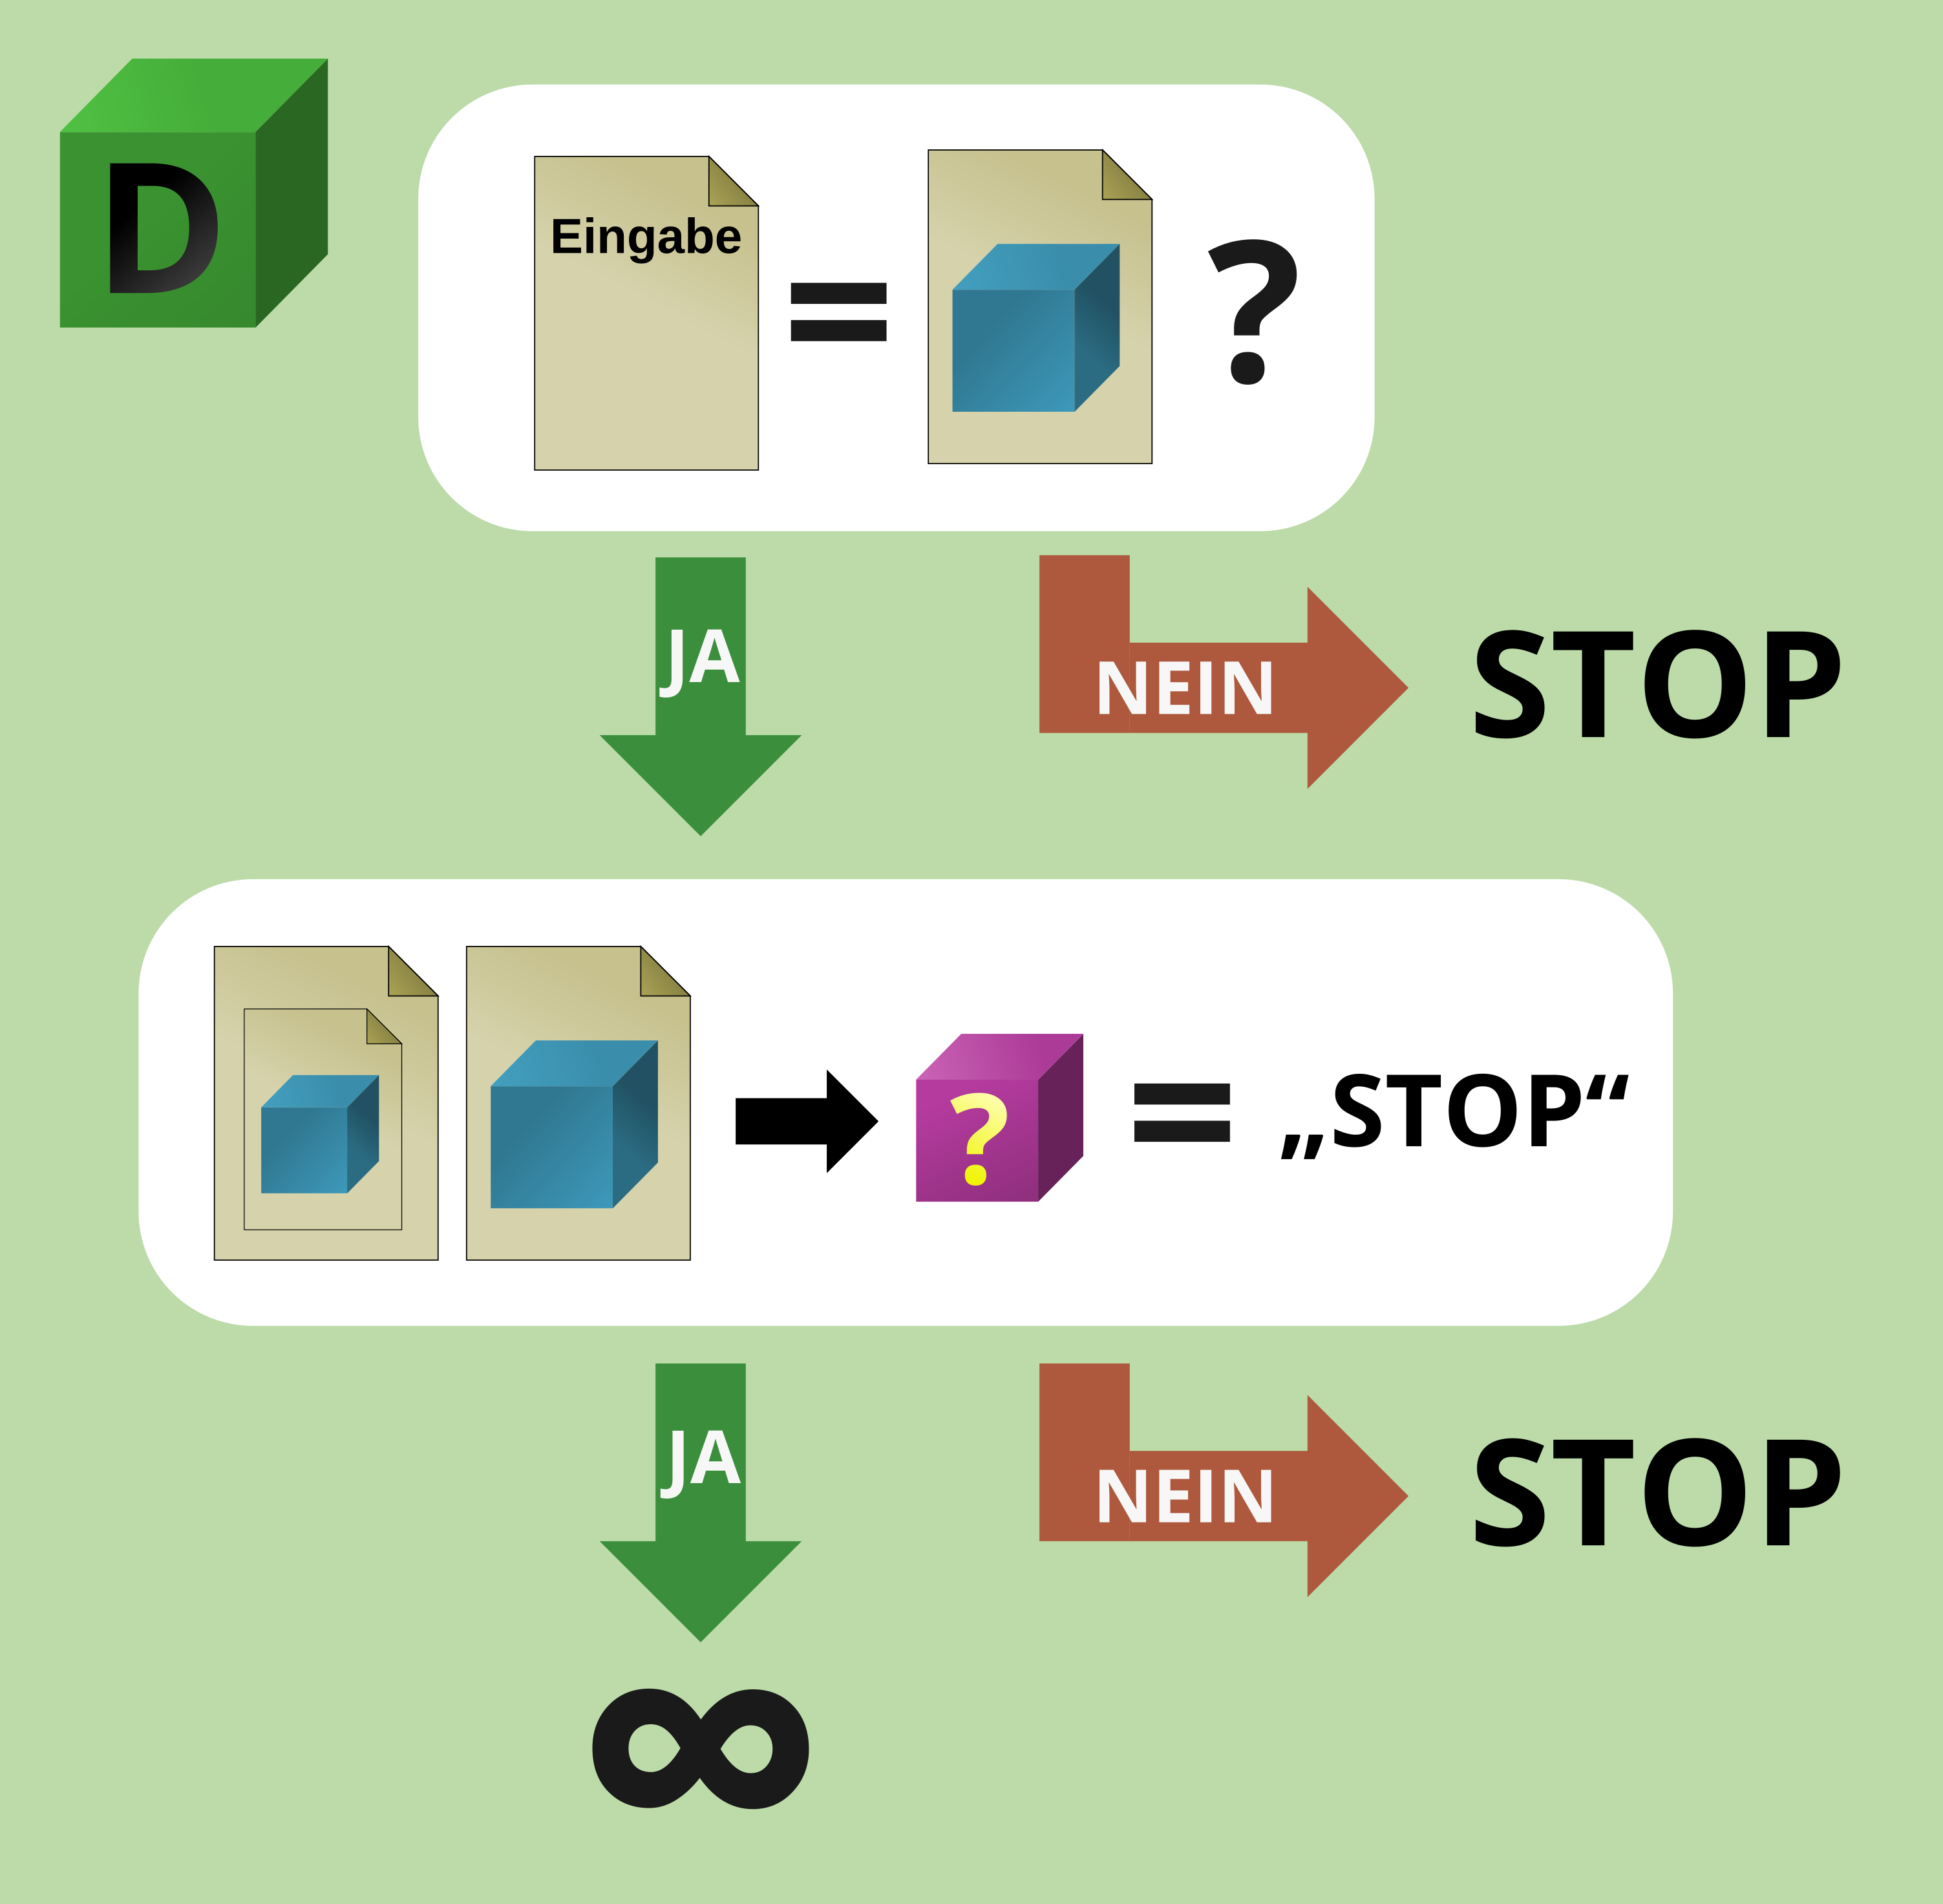
\includegraphics[height=5cm]{images/halting-d}\bigskip

\emph{Paradoxon:}
~\hspace{0.5cm}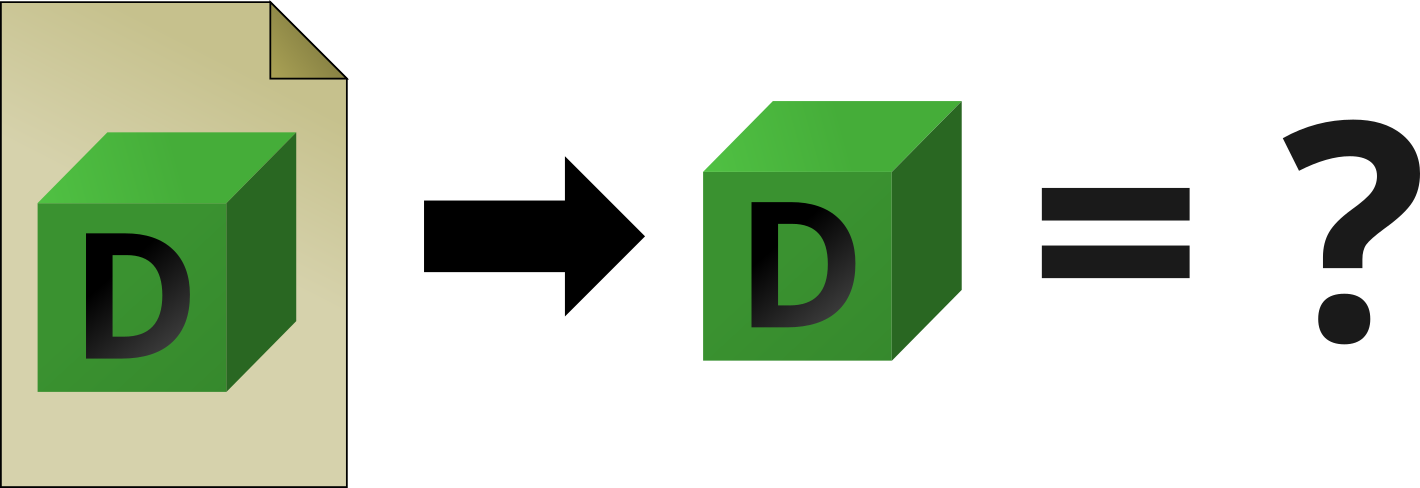
\includegraphics[height=1cm,valign=c]{images/halting-paradox}%\hfill~
\end{minipage}

\end{frame}

\begin{frame}[t]\frametitle{Beweis durch Reduktion\phantom{"`T"'}}

\theobox{\emph{Satz:} Das Halteproblem $\Slang{P}_{\textsf{Halt}}$ ist unentscheidbar.}\pause

\emph{Beweis:} Nehmen wir an, das Halteproblem wäre entscheidbar.\medskip\pause

Ein Algorithmus:
\begin{itemize}
\item Eingabe: (binärkodierte) natürliche Zahl $k$
\item Iteriere über alle Turingmaschinen $\Smach{M}$ mit $k$ Zuständen über dem Arbeitsalphabet $\{\Sterm{x},\blank\}$:
\begin{itemize}
\item Entscheide ob $\Smach{M}$ bei leerer Eingabe $\epsilon$ hält\\
{\footnotesize\textcolor{devilscss}{(möglich, wenn das Halteproblem entscheidbar ist)}}
\item Falls ja, dann simuliere $\Smach{M}$ auf der leeren Eingabe und zähle
		nach der Terminierung von $\Smach{M}$ die $\Sterm{x}$ auf dem Band\\
{\footnotesize\textcolor{devilscss}{(möglich, da es universelle Turingmaschinen gibt)}}
\end{itemize}
\item Ausgabe: die maximale Zahl der geschriebenen $\Sterm{x}$.
\end{itemize}\pause
Dieser Algorithmus würde die Busy-Beaver-Funktion $\bbfunc:\mathbb{N}\to\mathbb{N}$
berechnen.\medskip

Wir wissen, dass das unmöglich ist -- Widerspruch.\qed

\end{frame}

\begin{frame}\frametitle{Turing-Reduktionen}

Unser Beweis konstruiert den Algorithmus für ein Problem (Busy Beaver)
durch Aufruf von Subroutinen für ein anderes \ghost{(Halteproblem)}
\bigskip\pause

Diese Idee lässt sich verallgemeinern:

\defbox{Ein Problem $\Slang{P}$ ist \redalert{Turing-reduzierbar} auf ein Problem
$\Slang{Q}$ 
(in Symbolen: $\Slang{P}\leq_T \Slang{Q}$), wenn man $\Slang{P}$ mit einem Programm lösen
kann, welches ein Programm für $\Slang{Q}$ als Unterprogramm aufrufen darf.}

{\footnotesize
\emph{Anmerkung:} Das ist etwas informell. Eine ganz formelle Definition verwendet den Begriff des \alert{Orakels} für Turingmaschinen.
}\medskip\pause

\examplebox{\emph{Beispiel:} Unser Beweis basiert auf einer Turing-Reduktion der Berechnung der Busy-Beaver-Funktion auf das Halteproblem.}

\end{frame}

\begin{frame}\frametitle{Turing-Reduktionen: Beispiel}

\examplebox{\emph{Beispiel:} Das Nicht-Halteproblem $\overline{\Slang{P}}_{\textsf{Halt}}$,
ist definiert als\\[1ex]
\narrowcentering{$\overline{\Slang{P}}_{\textsf{Halt}} = \{\textsf{enc}(\Smach{M})\Sterm{\#}\Sterm{\#}\textsf{enc}(w)\mid \text{$\Smach{M}$ hält nicht bei Eingabe $w$}\}$}\\[1ex]
%
$\overline{\Slang{P}}_{\textsf{Halt}}$ ist Turing-reduzierbar auf $\Slang{P}_{\textsf{Halt}}$: (1) Prüfe Eingabeformat, (2) entscheide Halteproblem, (3) invertiere Ergebnis.\\[1ex]

Analog kann auch $\Slang{P}_{\textsf{Halt}}$ auf $\overline{\Slang{P}}_{\textsf{Halt}}$ Turing-reduziert werden.}\bigskip\pause

Daraus ergibt sich:\medskip

\theobox{\emph{Satz:} Das Nicht-Halteproblem $\overline{\Slang{P}}_{\textsf{Halt}}$ ist unentscheidbar.}

\end{frame}

\begin{frame}\frametitle{$\epsilon$-Halten}

Sonderfälle des Halteproblems sind in der Regel nicht einfacher:\medskip

\defbox{Das \redalert{$\epsilon$-Halteproblem} besteht in der folgenden Frage:\\
\hspace{1cm}Gegeben eine TM $\Smach{M}$,\\\hspace{1cm} wird $\Smach{M}$ für die leere Eingabe $\epsilon$ jemals anhalten?}\medskip\pause

\theobox{\emph{Satz:} Das $\epsilon$-Halteproblem ist unentscheidbar.}\pause

\emph{Beweis:} Angenommen das Problem wäre entscheidbar.\medskip

Ein Algorithmus:
\begin{itemize}
\item Eingabe: Eine Turingmaschine $\Smach{M}$ und ein Wort $w$.
\item Konstruiere eine TM $\Smach{M}_w$, die zwei Schritte ausführt:
	\begin{enumerate}[(1)]
	\item Lösche das Eingabeband und fülle es mit dem Wort $w$
	\item Verarbeite diese Eingabe wie $\Smach{M}$ 
	\end{enumerate}
\item Entscheide das $\epsilon$-Halteproblem für $\Smach{M}_w$.
\item Ausgabe: Ergebnis des $\epsilon$-Halteproblems
\end{itemize}\pause

Dies würde das Halteproblem entscheiden -- Widerspruch. \qed

\end{frame}

\begin{frame}\frametitle{Beweistechniken im Vergleich}

Wir haben zwei ähnliche Unentscheidbarkeitsbeweise gesehen:\bigskip

\begin{minipage}{5cm}
\alert{Halteproblem}
\begin{itemize}
\item Reduktion der Busy-Beaver-Funktion
\item Algorithmus ruft Subroutine für Halteproblem exponentiell oft auf
\item Ausgabe wird durch weitere TM-Simulationen berechnet
\end{itemize}\bigskip
~\hspace{5mm}$\leadsto$ Turing-Reduktion!
\end{minipage}%
\begin{minipage}{5cm}
\alert{$\epsilon$-Halteproblem}
\begin{itemize}
\item Reduktion des Halteproblems
\item Algorithmus ruft Subroutine für $\epsilon$-Halteproblem immer genau einmal auf
\item Ausgabe ist das Ergebnis der $\epsilon$-Halteproblem-Routine
\end{itemize}\bigskip
~\hspace{5mm}$\leadsto$ Turing-Reduktion?
\end{minipage}

\end{frame}

\begin{frame}\frametitle{Many-One-Reduktionen}

\emph{Idee:} Im letzten Beweis verwendeten wir das $\epsilon$-Halteproblem nicht als Subroutine eines komplexen Programms, sondern wir formten das Halteproblem in ein $\epsilon$-Halteproblem um\bigskip

\defbox{Eine berechenbare totale Funktion $f:\Sigma^*\to\Sigma^*$ ist eine \redalert{Many-One-Reduktion} von einer Sprache \Slang{P} auf eine Sprache \Slang{Q} (in Symbolen: $\Slang{P}\leq_m \Slang{Q}$), wenn für alle Wörter $w\in\Sigma^*$ gilt:\\[1ex]
\narrowcentering{$w\in\Slang{P}\quad$ genau dann wenn $\quad f(w)\in\Slang{Q}$}}\pause\bigskip

\examplebox{\emph{Beispiel:} Die folgende Funktion definiert eine Many-One-Reduktion vom
Halteproblem auf das $\epsilon$-Halteproblem:%\\%[-4ex]
\[f(v)=\left\{\begin{array}{ll}
\textsf{enc}(\Smach{M}_w) & \text{falls $v=\textsf{enc}(\Smach{M})\Sterm{\#\#}\textsf{enc}(w)$ für eine TM $\Smach{M}$}\\
\Sterm{\#} & \text{falls die Eingabe nicht korrekt kodiert ist}
\end{array}\right.\]
Dabei ist $\Smach{M}_w$ die TM aus dem Beweis.}

% \examplebox{Beispiel: Die Funktion $f$ mit $f(w)=w\Sterm{\#\#}\textsf{enc}(\epsilon)$ definiert eine Many-One-Reduktion vom
% $\epsilon$-Halteproblem auf das Halteproblem.}

\end{frame}

\begin{frame}\frametitle{Entscheidbarkeit durch Reduktion}

Das folgende Resultat drückt die wesentliche Idee hinter Reduktionen aus:\bigskip

\theobox{\emph{Satz:} Wenn $\Slang{P}\leq_m \Slang{Q}$ und $\Slang{Q}$ entscheidbar ist, dann ist
auch $\Slang{P}$ entscheidbar.}

\emph{Beweis:} Die Reduktion liefert einen Entscheidungsalgorithmus.\qed\bigskip\pause

Eigentlich benutzen wir bisher vor allem die Umkehrung:\bigskip

\theobox{\emph{Satz:} Wenn $\Slang{P}\leq_m \Slang{Q}$ und $\Slang{P}$ unentscheidbar ist, dann ist auch $\Slang{Q}$ unentscheidbar.}

\end{frame}

\begin{frame}\frametitle{Many-One vs. Turing}
\pause

Many-One-Reduktionen sind schwächer als Turing-Reduktionen:\bigskip

\theobox{\emph{Satz:} Jede Many-One-Reduktion kann als Turing-Reduktion ausgedrückt werden.}

\emph{Beweis:} Die Turing-Reduktion ergibt sich, wenn man die (berechenbare) Many-One-Reduktionsfunktion als Teil einer TM implementiert.\qed
\bigskip\pause

\theobox{\emph{Satz:} Es gibt Probleme $\Slang{P}$ und $\Slang{Q}$, für die $\Slang{P}\leq_T \Slang{Q}$ gilt, aber nicht $\Slang{P}\leq_m \Slang{Q}$.}

\emph{Beweis:} Wir haben bereits gesehen, dass $\Slang{P}_{\textsf{Halt}}\leq_T\overline{\Slang{P}}_{\textsf{Halt}}$. Aber es gilt nicht $\Slang{P}_{\textsf{Halt}}\leq_m\overline{\Slang{P}}_{\textsf{Halt}}$ -- wir werden in der nächsten Vorlesung sehen, warum nicht.\qed

\end{frame}

% \begin{frame}\frametitle{Äquivalenz von Turingmaschinen}
% 
% Hier noch ein Beispiel für eine Many-One-Reduktion:
% 
% \defbox{Zwei Turingmaschinen $\Smach{M}_1$ und $\Smach{M}_2$ sind \redalert{äquivlent}, wenn sie die gleiche Sprache akzeptieren.}\medskip
% 
% \theobox{Satz: Äquivalenz von Turingmaschinen ist nicht entscheidbar.}
% 
% \emph{Beweis:} 
% 
% \end{frame}



\begin{frame}\frametitle{Zusammenfassung und Ausblick}

LOOP-Programme können wirklich fast alle praktisch relevanten Probleme lösen
\bigskip

Durch Reduktionen können wir aus der (Un)Lösbarkeit eines Problems die (Un)Lösbarkeit eines anderen ableiten\bigskip

Turing-Reduktionen $\Slang{P}\leq_T\Slang{Q}$ verwenden die Lösung von $\Slang{Q}$ als Subroutine in einem Algorithmus für $\Slang{P}$
\bigskip

Many-One-Reduktionen $\Slang{P}\leq_m\Slang{Q}$ formen eine Problemstellung für $\Slang{P}$ in eine Problemstellung für $\Slang{Q}$ um
\bigskip

\anybox{yellow}{
Was erwartet uns als nächstes?
\begin{itemize}
\item Mehr zu Semi-Entscheidbarkeit 
\item Ein unentscheidbares Problem von Emil Post \ldots
\item \ldots{} und unendlich viele von Henry Gordon Rice 
\end{itemize}
}

\end{frame}

% \begin{frame}[t]\frametitle{Bildrechte}
% 
% Folie \ref{frame_hilbert}: gemeinfrei\\
% Folie \ref{frame_cantor}: Fotografie von 1870, gemeinfrei\\
% Folie \ref{frame_rado}: Ausschnitt aus einer Fotografie von 1928, \url{http://www.bibl.u-szeged.hu/sztegy/photo/778.jpg}, CC-By-SA 3.0\\
% 
% \end{frame}


\end{document}
